\part{Algorithms}
	\chapter{Computational Complexity}
		\section{Asymptotic Notation}
			\subsection{Asymptotic Analysis}
				\begin{definition}[asymptotically positive function]
					$f: \mathbb{N} \rightarrow \mathbb{R}$ is an asymptotically positive function if $\exists n_0 > 0$ such that $\forall n > n_0$ we have $f(n) > 0$
				\end{definition}

			\subsection{\texorpdfstring{$O$}{O}-Notation, \texorpdfstring{$\Omega$}{Omega}-Notation and \texorpdfstring{$\Theta$}{Theta}-Notation}
				\begin{definition}[$O$-Notation]
					For a function $g(n)$, $O(g(n)) = \{f: \exists c > 0, n_0 > 0 \text{ such that } f(n) \le cg(n), \forall n\ge n_0\}$
				\end{definition}
				$O$-Notation also known as asymptotic upper bound. 

				\begin{definition}[$\Omega$-Notation]
					For a function $g(n)$, $\Omega(g(n)) = \{f: \exists c > 0, n_0 > 0 \text{ such that } f(n) \ge cg(n), \forall n\ge n_0\}$
				\end{definition}
				$\Omega$-Notation also known as asymptotic lower bound.

				\begin{definition}[$\Theta$-Notation]
					For a function $g(n)$, $\Theta(g(n)) = \{f: \exists c > 0, n_0 > 0 \text{ such that }  c_1g(n) \le f(n) \le c_2g(n), \forall n\ge n_0\}$
				\end{definition}
				$\Omega$-Notation and $\Theta$-Notation are not used very often when we talk about running times.

				\begin{definition}[$o$-Notation]
					For a function $g(n)$, $o(g(n)) = \{f: \exists c > 0, n_0 > 0 \text{ such that } f(n) <\le> cg(n), \forall n\ge n_0\}$
				\end{definition}

				\begin{definition}[$\omega$-Notation]
					For a function $g(n)$, $\omega(g(n)) = \{f: \exists c > 0, n_0 > 0 \text{ such that } f(n) > cg(n), \forall n\ge n_0\}$
				\end{definition}

				\notice{$O(g)$, $\Omega(g)$ and $\Theta(g)$ are sets, we use ``$=$'' to represent ``$\in$''. In here ``$=$'' is asymmetric. Equality such as $O(n^3) = n^3 + n$ is incorrect.}

				\begin{example}
					The following are some examples
					\begin{align}
						\centering
						\begin{tabular}{|c|c||c|c|c|}
							\hline
							$f(n)$ & $g(n)$ & $O$ & $\Omega$ & \Theta\\
							\hline
							$4n^2 + 3n$ & $n^3 - 2n + 3$ & Yes & No & No \\
							\hline
							$\lg^{10} n$ & $n^{0.1}$ & Yes & No & No \\
							\hline
							$\log_{10} n$ & \lg(n^3) & Yes & Yes & Yes \\
							\hline
							$\lceil \sqrt{10n + 100} \rceil$ & $n$ & Yes & No & No \\
							\hline
							$n^3 -100n$ & $10n^2\lg n$ & No & Yes & No\\
							\hline
							$2^n$ & 2^{\frac n2} $ & No & Yes & No \\
							\hline
							$\sqrt{n}$ & n^{\sin n} & No & No & No\\
							\hline
						\end{tabular}
					\end{align}
				\end{example}

				\begin{theorem}
					Let $f$ and $g$ be two functions that
					\begin{equation}
						\lim_{n\rightarrow \infty} \frac{f(n)}{g(n)} = c > 0
					\end{equation}
					Then $f(n) = \Theta(g(n))$
				\end{theorem}

				\begin{proof}
					Since $\lim_{n\rightarrow \infty} \frac{f(n)}{g(n)}$ exists and positive, there is some $n_0$ beyond which the ratio is always between $\frac12 c$ and 2c. Thus,
					\begin{align}
						& \forall n > n_0, f(n) \le 2cg(n) \Rightarrow f(n) = O(g(n)) \\
						& \forall n > n_0, f(n) \ge \frac12cg(n) \Rightarrow f(n) = \Omega(g(n))
					\end{align}
				\end{proof}

				A set of properties:
				\begin{align}
					& f(n) = O(g(n)) \iff g(n) = \Omega(f(n))\\
					& f(n) = \Theta(g(n)) \iff f(n) = O(g(n)) \text{ and } g(n) = O(f(n))
				\end{align}

				Another set of properties:
				\begin{align}
					& f = O(g), g = O(h) \Rightarrow f=O(h) \\
					& f = \Omega(g), g = \Omega(h) \Rightarrow f=\Omega(h) \\
					& f = \Theta(g), g = \Theta(h) \Rightarrow f=\Theta(h)
				\end{align}

				\begin{theorem}
					If $f_i = O(h)$, for finite number of $i \in K$, then $\sum_{i\in K} f_i = O(h)$
				\end{theorem}

				Proof is trivia.

				\notice{Function $f$ and $g$ not necessarily have relation $f=O(g)$ or $g=O(f)$. E.g., for $f = \sqrt{n}$ and $g = n^{\sin n}$, $f \notin O(g)$ and $g \notin O(f)$ }

		\section{Common Running Times}
			\subsection{\texorpdfstring{$O(n)$}{O(n)}}
				\begin{example}
					Scan through a list to find a element matching with input
				\end{example}

			\subsection{\texorpdfstring{$O(\lg n)$}{O(lgn)}}
				\begin{example}
					Binary-search
				\end{example}

			\subsection{\texorpdfstring{$O(n^2)$}{O(n2)}}
				\begin{example}
					Scan through every pair of elements, $\binom{n}{2}$
				\end{example}

			\subsection{\texorpdfstring{$O(n^3)$}{O(n3)}}
				\begin{example}
					Matrix-multiplication by definition
				\end{example}

			\subsection{\texorpdfstring{$O(n\lg n)$}{O(nlgn)}}
				\begin{example}
					Many divide and conquer algorithm which in each step iteratively divide the problem into two part and solve the sub-problem, for example merge-sort.
				\end{example}

			\subsection{\texorpdfstring{$O(n!)$}{O(n!)}}
				\begin{example}
					Enumerate all permutation, for example Hamiltonian Cycle Problem
				\end{example}

			\subsection{\texorpdfstring{$O(c^n)$}{O(cn)}}
				\begin{example}
					Enumerate all elements in power set. ($O(2^n)$)
				\end{example}

			\subsection{\texorpdfstring{$O(n^n)$}{O(nn)}}
				\begin{example}
					Enumerate all combinations. (Can't find good example yet)
				\end{example}

			\subsection{Comparison between Running Times}
				$\lg n < n < n\lg n < n^2 < n^{\sqrt{n}} < 2^n < e^n < n! < n^n$

	\chapter{General Strategies}
		\section{Greedy Algorithms}

		\section{Divide and Conquer}

		\section{Dynamic Programming}

	\chapter{Sorting}
		\section{Bubble Sort}

		\section{Insertion Sort}

		\section{Selection Sort}

		\section{Heap-sort}

		\section{Quick-sort}

		\section{Merge-sort}

		\section{Sorting in Linear Time}

	\chapter{Mathematical Algorithm}
		\section{Matrices Multiplication}

		\section{Gaussian Elimination}

		\section{Curve Fitting}

		\section{Integration}

		\section{}

	\chapter{Searching}

	\chapter{String}
		\section{String Searching}

		\section{Pattern Matching}

		\section{Parse}

		\section{File Compression}

		\section{Cryptology}

	\chapter{Geometric Algorithm}
		\section{Convex Hull}

		\section{Geometric Intersection}

		\section{Closest Point}

		\section{Polygon Triangulation}
			\subsection{Types of Polygons}
				\begin{definition}[simple polygon]
					A \textbf{simple polygon} is a closed polygonal curve without self-intersection.
				\end{definition}

				\begin{figure}[h!]
					\centering
					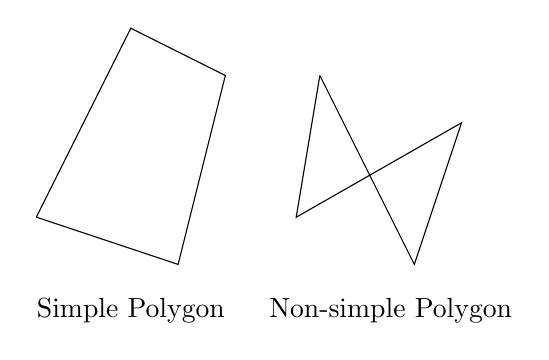
\begin{tikzpicture}[scale=0.6]
						\draw (0, 0) -- (3, -1) -- (4, 3) -- (2, 4) -- (0, 0);
						\draw (6, 3) -- (8, -1) -- (9, 2) -- (5.5, 0) -- (6, 3);
						\node at (2, -1.5) [below] {Simple Polygon};
						\node at (7.5, -1.5) [below] {Non-simple Polygon};
					\end{tikzpicture}
				\end{figure}

				Polygons are basic building blocks in most geometric applications. It can model arbitrarily complex shapes, and apply simple algorithms and algebraic representation/manipulation.

			\subsection{Triangulation}
				\begin{definition}[Triangulation]
					\textbf{Triangulation} is to partition polygon $P$ into non-overlapping triangles using diagonals only. It reduces complex shapes to collection of simpler shapes. Every simple $n$-gon admits a triangulation which has $n-2$ triangles.				
				\end{definition}

				\begin{figure}[h!]
					\centering
					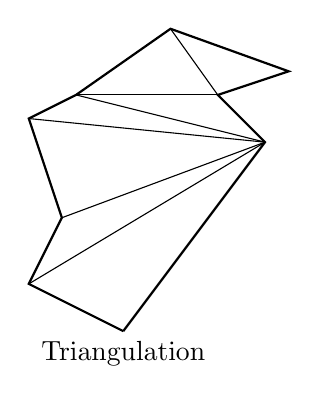
\begin{tikzpicture}[scale=0.6]
						\draw [thick] (0, 0) -- (3, 4) -- (2, 5) -- (3.5, 5.5) -- (1, 6.4) -- (-1, 5) -- (-2, 4.5) -- (-1.3, 2.4) -- (-2, 1) -- (0, 0);
						\draw (-2, 1) -- (3, 4);
						\draw (-1.3, 2.4) -- (3, 4);
						\draw (-2, 4.5) -- (3, 4);
						\draw (-1, 5) -- (3, 4);
						\draw (-1, 5) -- (2, 5);
						\draw (2, 5) -- (1, 6.4);
						\node at (0, 0) [below] {Triangulation};
					\end{tikzpicture}
				\end{figure}

				\begin{theorem}
					Every polygon has a triangulation				
				\end{theorem}

				\begin{lemma}
					Every polygon with more than three vertices has a diagonal.
				\end{lemma}

				\begin{proof}
					(by Meisters, 1975) Let $P$ be a polygon with more than three vertices. Every vertex of a $P$ is either \textit{convex} or \textit{concave}. W.L.O.G.(any polygon must has convex corner) Assume $p$ is a convex vertex. Denote the neighbors of $p$ as $q$ and $r$. If $\bar{qr}$ is a diagonal, done, and we call $\triangle{pqr}$ is an \textit{ear}. If $\triangle{pqr}$ is not an ear, it means at least one vertex is inside $\triangle{pqr}$, assume among those vertexes inside $\triangle{pqr}$, $s$ is a vertex closest to $p$, then $\bar{ps}$ is a diagonal.
				\end{proof}

			\subsection{Art Gallery Theorem}
				\begin{theorem}
					Every $n$-gon can be guarded with $\lfloor \frac{n}{3} \rfloor$ vertex guards
				\end{theorem}

				\begin{lemma}
					Triangulation graph can be 3-colored.
				\end{lemma}

				\begin{problem}
					The floor plan of an art gallery modeled as a simple polygon with $n$ vertices, there are guards which is stationed at fixed positions with 360 degree vision but cannot see through the walls. How many guards does the art gallery need for the security? (Fun fact: This problem was posted to Vasek Chvatal by Victor Klee in 1973).				
				\end{problem}

				\begin{proof}
					- $P$ plus triangulation is a planar graph\\
					- 3-coloring means there exist a 3-partition for vertices that no edge or diagonal has both endpoints within the same set of vertices.\\
					- Proof by Induction:\\
					\indent - Remove an ear (there will always exist ear) \\
					\indent - Inductively 3-color the rest\\
					\indent - Put ear back, coloring new vertex with the label not used by the boundary diagonal.
				\end{proof}

			\subsection{Triangulation Algorithms}

	\chapter{Data Structures}
		\section{Elementary Data Structures}

		\section{Hash Tables}

		\section{Binary Search Trees}

		\section{Red-Black Trees}

		\section{B-Trees}

		\section{Fibonacci Heaps}

		\section{van Emde Boas Trees}

	\chapter{NP and PSPACE}


				\begin{algorithm}[h!]
					\caption{Simplex Method}
					\begin{algorithmic}[1]
						\REQUIRE Given a basic feasible solution with basis $B$
						\ENSURE Optimal objective value $\min z= cx$
						\STATE Set $\mathbf{B}$ for basic variables, $\mathbf{N}$ for nonbasic variables
						\STATE $\mathbf{B} \gets \text{all slack variables}$
						\STATE $\mathbf{N} \gets \text{all variables excepts slack variables}$
						\FOR{$\forall j$}
							\STATE $z_j=c_BB^{-1}a_j=0$
						\ENDFOR
						\WHILE{$\exists z_j-c_j > 0$}
							\STATE $z_j=wa_j-c_j=c_BB^{-1}a_j-c_j$
							\STATE $z_k-c_k=\max\limits_{j \in \mathbf{N}}\{z_j-c_j\}$
							\STATE $y_k=B^{-1}a_k$
							\IF{$\exists y_{ik} >0$}
								\STATE $\theta_r=\min\limits_{i \in \mathbf{B}}\{\theta_i=\frac{\bar{b}_i}{y_{ik}}:y_{ik}>0\}$
								\STATE $\mathbf{B} \gets \mathbf{B} \backslash \{k\}$
								\STATE $\mathbf{N} \gets \mathbf{N} \cup \{k\}$
								\STATE $\mathbf{B} \gets \mathbf{B} \cup \{r\}$
								\STATE $\mathbf{N} \gets \mathbf{N} \backslash \{r\}$
							\ELSE
								\STATE Unbounded
							\ENDIF
						\ENDWHILE
						\STATE $x_B^*=B^{-1}b=\bar{b}$
						\STATE $x_N=0$
						\STATE $z^*=c_BB^{-1}b=c_B\bar{b}\mathbf{a_{B_k}}$
					\end{algorithmic}
				\end{algorithm}